% 第3章第6节：空间离散与数值解（有限差分与网格方程；Galerkin与有限元方法；时间推进与误差分配）。

\section{空间离散与数值解}
\label{sec:pde-discretization}

前面各节研究的是连续的场。计算机只能存储有限个数，所以要把场换成有限个未知量，把偏微分方程换成代数方程或常微分方程组。本节固定前面的方程和数据，研究两种空间离散：有限差分在网格点上逼近导数，有限元在有限维函数子空间上求弱形式。演化问题经空间离散后变成常微分方程组，再用第~\ref{chap:ordinary-differential-equations}章的时间推进方法求解。我们始终区分三个误差来源：空间离散的误差、时间推进的误差和代数方程没有解准的误差。

\subsection{有限差分与网格方程}
\label{sec:pde-finite-difference}

\paragraph{差商与网格未知量}
在$[0,1]$上取等距网格$x_j=jh$，$j=0,1,\ldots,N+1$，$h=1/(N+1)$。两端$x_0,x_{N+1}$是边界点，值由边界条件给出；内部的$N$个未知数$U_j$是对$u(x_j)$的近似。\term{有限差分方法}（finite difference method）把导数换成网格值的差商。对二阶导数，用中心差商
\[
  \delta_h^2u(x)=\frac{u(x+h)-2u(x)+u(x-h)}{h^2} .
\]
设$u\in C^4$，把$u(x\pm h)$在$x$处展开到四阶并带Lagrange余项，奇数阶项相互抵消，两个四阶余项由介值定理合并，得
\begin{equation}
  \delta_h^2u(x)=u''(x)+\frac{h^2}{12}u^{(4)}(\xi),\qquad\xi\in(x-h,x+h).
  \label{eq:pde-central-difference}
\end{equation}
差商以$h^2$的速度逼近二阶导数。这与式~\eqref{eq:pde-neighbor-average}是同一件事：二阶导数度量一点与两侧邻居平均值之差。

\paragraph{Poisson方程的网格方程}
对$-u''=f$、$u(0)=\alpha$、$u(1)=\beta$，在每个内部网格点上用差商代替二阶导数：
\[
  \frac{-U_{j-1}+2U_j-U_{j+1}}{h^2}=f(x_j),\qquad j=1,\ldots,N,\qquad U_0=\alpha,\ U_{N+1}=\beta .
\]
第一个和最后一个方程含有已知的边界值，把它们移到右端：第$1$行的右端变为$f(x_1)+\alpha/h^2$，第$N$行变为$f(x_N)+\beta/h^2$。记$\bm U=(U_1,\ldots,U_N)^{\top}$，得到线性方程组
\begin{equation}
  \bm A_h\bm U=\bm F,\qquad
  \bm A_h=\frac1{h^2}\begin{bmatrix}2&-1&&\\-1&2&\ddots&\\&\ddots&\ddots&-1\\&&-1&2\end{bmatrix}\in\mathbb R^{N\times N}.
  \label{eq:pde-fd-poisson}
\end{equation}
$\bm A_h$是对称三对角矩阵，每行至多三个非零元，共$3N-2$个；用三对角消元求解只需$O(N)$次运算。在单位正方形上用$N\times N$个内部网格点，五点格式$(4U_{i,j}-U_{i-1,j}-U_{i+1,j}-U_{i,j-1}-U_{i,j+1})/h^2=f_{i,j}$给出$N^2$个未知数，每行至多五个非零元。图~\ref{fig:pde-fd-stencil-sparsity}画出了一维模板和两种矩阵的非零元位置：矩阵很大，但几乎全是零。

\begin{figure*}[!htb]
  \centering
  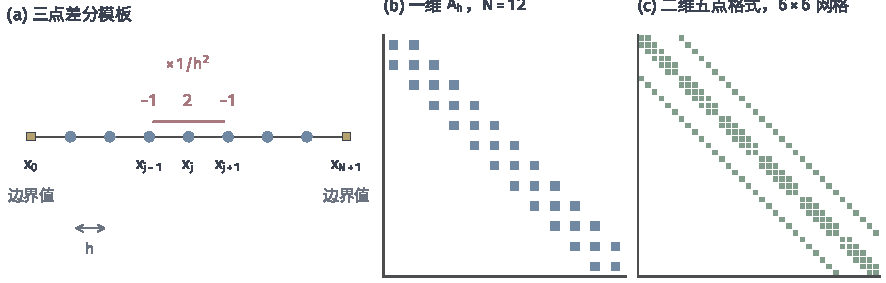
\includegraphics[width=150mm]{figures/03-optimization-evolution-and-signals/02-processes-and-trajectory-evolution/matplotlib/pde-fd-stencil-sparsity/figure.pdf}
  \caption{有限差分的网格与矩阵结构。(a)~一维网格：方块为已知的边界值，圆点为未知数；第$j$个方程用$x_{j-1},x_j,x_{j+1}$三点，权重为$(-1,2,-1)/h^2$。(b)~一维矩阵$\bm A_h$的非零元，$N=12$，三对角。(c)~单位正方形上$6\times6$内部网格的五点格式按行编号后的$36\times36$矩阵：主对角线两侧各有一条紧邻的副对角线（同一行的左右邻居）和一条相距$6$的副对角线（上下邻居）。}
  \label{fig:pde-fd-stencil-sparsity}
\end{figure*}

$\bm A_h$的特征向量可以直接写出。令$(\bm v_k)_j=\sin(k\pi x_j)$，$k=1,\ldots,N$。由$\sin(k\pi(x_j+h))+\sin(k\pi(x_j-h))=2\cos(k\pi h)\sin(k\pi x_j)$，且$\sin(k\pi x_0)=\sin(k\pi x_{N+1})=0$，
\[
  \bm A_h\bm v_k=\mu_k\bm v_k,\qquad\mu_k=\frac{2-2\cos(k\pi h)}{h^2}=\frac4{h^2}\sin^2\frac{k\pi h}{2} .
\]
离散的特征向量正是连续模式$\sin(k\pi x)$在网格上的取样。低频时$\mu_k\approx k^2\pi^2$，与连续的特征值一致；最高频$\mu_N\approx4/h^2$，远小于连续的$N^2\pi^2\approx\pi^2/h^2$，网格无法如实表示比两倍网格间距更短的波长。最大与最小特征值之比约为$4/(\pi^2h^2)$，网格越细，矩阵的条件数越大。

\paragraph{一致性：截断误差}
网格解$\bm U$离精确解有多远？第一步是问：把精确解代入网格方程，差多少。设$u\in C^4$是精确解，定义\term{截断误差}（truncation error）$\tau_j=(\bm A_h\bm u_h)_j-F_j$，其中$\bm u_h=(u(x_1),\ldots,u(x_N))^{\top}$。由式~\eqref{eq:pde-central-difference}与$-u''=f$，
\[
  \tau_j=-\delta_h^2u(x_j)+u''(x_j)=-\frac{h^2}{12}u^{(4)}(\xi_j),\qquad\|\bm\tau\|_\infty\leq\frac{h^2}{12}\|u^{(4)}\|_\infty .
\]
截断误差趋于零，称格式与方程一致。但这只说明精确解“几乎满足”网格方程，并没有说明网格方程的解接近精确解：若$\bm A_h^{-1}$的范数随$h\to0$无界增长，很小的$\bm\tau$也可能被放大成很大的误差。还需要一个与$h$无关的稳定估计。

\paragraph{稳定性：离散最大值原理}
连续问题有最大值原理，网格方程也有。

\begin{lemma}[离散最大值原理]
\label{lem:pde-discrete-max}
设$\bm V\in\mathbb R^N$，补充$V_0=V_{N+1}=0$。若$(\bm A_h\bm V)_j\geq0$对所有$j$成立，则$\bm V\geq\bm 0$（逐分量）。因此$\bm A_h$可逆，且$\bm A_h^{-1}$的元素全部非负。
\end{lemma}

\begin{proof}
设$m=\min_jV_j$在$j_*$处取到，反设$m<0$。由$(\bm A_h\bm V)_{j_*}\geq0$，$2m=2V_{j_*}\geq V_{j_*-1}+V_{j_*+1}\geq2m$，等号成立，两个邻居也等于$m$。逐步向左推，直到$j=1$：它的左邻居$V_0=0$也必须等于$m<0$，矛盾。所以$\bm V\geq\bm 0$。若$\bm A_h\bm V=\bm 0$，对$\bm V$与$-\bm V$分别使用结论得$\bm V=\bm 0$，$\bm A_h$可逆；对$\bm G\geq\bm 0$，$\bm V=\bm A_h^{-1}\bm G$满足条件，所以$\bm A_h^{-1}\bm G\geq\bm 0$。
\end{proof}

要得到定量的界，用一个比较函数。$w(x)=x(1-x)/2$是二次函数，式~\eqref{eq:pde-central-difference}中的余项为零，所以它的网格值$\bm w$精确满足$\bm A_h\bm w=\bm 1$，$\bm 1$为全一向量。对任意$\bm G$，向量$\|\bm G\|_\infty\bm w-\bm A_h^{-1}\bm G$经$\bm A_h$作用后为$\|\bm G\|_\infty\bm 1-\bm G\geq\bm 0$，由引理~\ref{lem:pde-discrete-max}它非负；同理$\|\bm G\|_\infty\bm w+\bm A_h^{-1}\bm G\geq\bm 0$。于是
\begin{equation}
  \|\bm A_h^{-1}\bm G\|_\infty\leq\|\bm G\|_\infty\max_jw_j\leq\frac18\|\bm G\|_\infty .
  \label{eq:pde-fd-stability}
\end{equation}
常数$1/8$与$h$无关。它是连续估计“$-u''=f$、两端为零时$\|u\|_\infty\leq\|f\|_\infty/8$”在网格上的复制品。

\paragraph{收敛：一致性加稳定性}
把两步合起来。误差$\bm e=\bm u_h-\bm U$满足$\bm A_h\bm e=\bm A_h\bm u_h-\bm F=\bm\tau$，由式~\eqref{eq:pde-fd-stability}得到下面的结论。

\begin{theorem}[一维Poisson差分格式的收敛]
\label{thm:pde-fd-convergence}
设$f$连续，$-u''=f$配Dirichlet边界条件的解$u\in C^4([0,1])$，$\bm U$为网格方程~\eqref{eq:pde-fd-poisson}的解。则
\[
  \max_{1\leq j\leq N}|u(x_j)-U_j|\leq\frac{h^2}{96}\|u^{(4)}\|_\infty .
\]
\end{theorem}

以$u=\sin(\pi x)$、$f=\pi^2\sin(\pi x)$为例，界为$\pi^4h^2/96\approx1.01h^2$。$N=4$、$h=0.2$时实际最大误差约$0.032$，界为$0.041$。图~\ref{fig:pde-convergence}中蓝色折线是$N$从$4$到$256$的实际误差，在对数坐标下斜率为$2.00$，与定理给出的阶一致。“一致性加稳定性推出收敛”是数值分析的一般原理；对线性问题，Lax等价定理把它表述为：一致的格式收敛当且仅当它稳定。这里的稳定性属于具体的格式与具体的范数，换一个格式或换一个范数需要重新证明。

\paragraph{热方程的半离散}
对热方程$u_t=\kappa u_{xx}+f$，只在空间上离散，时间保持连续：
\begin{equation}
  \bm U'(t)=-\kappa\bm A_h\bm U(t)+\bm F(t),\qquad\bm U(0)=\bigl(u_0(x_1),\ldots,u_0(x_N)\bigr)^{\top}.
  \label{eq:pde-semidiscrete-heat}
\end{equation}
这是一个$N$维线性常微分方程组，这种先离散空间、再处理时间的做法称为\term{方法线}（method of lines）。它的第$k$个特征分量以速率$\kappa\mu_k$衰减：低频模式的衰减率接近连续的$\kappa k^2\pi^2$，高频模式的衰减率被低估，但它们本来就在极短时间内衰减殆尽。空间误差就是半离散系统与连续解之差，下一小节在具体例子中把它与时间误差分开。

\subsection{Galerkin与有限元方法}
\label{sec:pde-fem}

有限差分直接逼近方程中的导数，要求解足够光滑才能用Taylor展开估计误差。另一条路线从弱形式出发：不逼近方程，而是在一个有限维函数空间中求弱形式的解。这条路线天然适合粗糙数据和不规则区域，误差分析也直接建立在第~\ref{sec:pde-poisson}节的能量框架上。

\paragraph{在有限维子空间上求弱形式}
设$V_h\subset H_0^1(\Omega)$是有限维子空间。\term{Galerkin方法}（Galerkin method）求$u_h\in V_h$，使
\begin{equation}
  a(u_h,v_h)=\ell(v_h)\qquad\text{对所有}v_h\in V_h .
  \label{eq:pde-galerkin}
\end{equation}
它只是把弱形式~\eqref{eq:pde-weak-dirichlet}中的解空间和检验空间同时换成$V_h$。取$V_h$的基$\varphi_1,\ldots,\varphi_n$，写$u_h=\sum_jc_j\varphi_j$，并依次取$v_h=\varphi_i$，得到线性方程组
\[
  \bm K\bm c=\bm F,\qquad\bm K_{i,j}=a(\varphi_j,\varphi_i),\qquad\bm F_i=\ell(\varphi_i).
\]
对Poisson方程，$\bm c^{\top}\bm K\bm c=a(v_h,v_h)=\|\nabla v_h\|^2>0$对非零的$v_h=\sum c_j\varphi_j$成立，$\bm K$对称正定，方程组有唯一解。由第~\ref{sec:pde-weak-form}小节的能量对应，$u_h$也是能量$J$在$V_h$上的最小点，这时称为Ritz方法；在有限维中求二次函数的最小点是第~\ref{chap:optimization}章已经处理过的问题。新的问题是：$u_h$与真正的解$u$相差多少。

\paragraph{帽函数与刚度矩阵}
一维时取与上一小节相同的网格，令
\[
  \varphi_j(x)=\max\Bigl(0,\,1-\frac{|x-x_j|}{h}\Bigr),\qquad j=1,\ldots,N .
\]
$\varphi_j$是在$x_j$处取$1$、在其余网格点取$0$、在每个小区间上线性的\term{帽函数}（hat function）。它们张成的$V_h$恰好是两端为零的连续分片线性函数全体，并且$v_h=\sum_jv_h(x_j)\varphi_j$：系数就是网格点上的值。用分片多项式基构造Galerkin空间的方法称为\term{有限元方法}（finite element method）。

两个帽函数只有在相邻时支撑才重叠，所以矩阵是三对角的。$\varphi_j'$在$(x_{j-1},x_j)$上为$1/h$、在$(x_j,x_{j+1})$上为$-1/h$，直接积分得$\bm K_{j,j}=2/h$、$\bm K_{j,j\pm1}=-1/h$，即\term{刚度矩阵}（stiffness matrix）$\bm K=h\bm A_h$。若把载荷$\bm F_i=\int f\varphi_i$近似为$f(x_i)\int\varphi_i=hf(x_i)$，方程$\bm K\bm c=\bm F$就变成$\bm A_h\bm c=(f(x_i))_i$，与有限差分格式~\eqref{eq:pde-fd-poisson}完全相同。两种方法出发点不同，在这个最简单的情形中给出同一组方程；区别在于有限元的误差分析来自弱形式，可以直接推广到粗糙数据、非均匀网格和高维的三角形网格。图~\ref{fig:pde-fem-hats}(a)画出了$h=1/6$时的五个帽函数。

\begin{figure}[!htb]
  \centering
  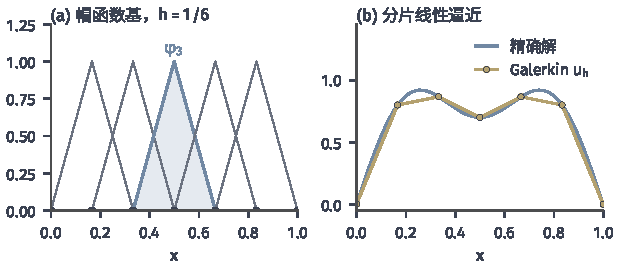
\includegraphics[width=105mm]{figures/03-optimization-evolution-and-signals/02-processes-and-trajectory-evolution/matplotlib/pde-fem-hats/figure.pdf}
  \caption{一维有限元。(a)~$h=1/6$时的帽函数基，蓝色阴影为$\varphi_3$，每个帽函数只与相邻两个重叠。(b)~$-u''=f$、两端为零的精确解$u=\sin(\pi x)+0.3\sin(3\pi x)$与Galerkin解$u_h$，载荷积分精确计算；$u_h$在网格点上与$u$相同（数值误差约$7\times10^{-10}$），在网格点之间线性插值。}
  \label{fig:pde-fem-hats}
\end{figure}

\paragraph{组装、边界条件与积分近似}
实际计算中，$\bm K$按单元逐块组装：在每个小区间上，两个局部基函数给出$2\times2$的单元矩阵$\tfrac1h\bigl[\begin{smallmatrix}1&-1\\-1&1\end{smallmatrix}\bigr]$，把它加到全局矩阵的对应位置即可。高维的三角形单元同样处理，只是单元矩阵由三角形的几何决定。

计算流程中的每一个环节对应一种近似，分别改变不同的对象。选$V_h$决定了用什么函数逼近解，这是空间离散。非零Dirichlet数据把边界节点的值固定，并把它们的贡献移到右端；Neumann数据则保留边界节点为未知数，把边界积分$\int g v_h$加入载荷，自然边界条件在这里不需要额外处理。用数值积分计算$\bm F_i$或$\bm K_{i,j}$，相当于把$\ell$或$a$换成近似的$\ell_h$或$a_h$，解的是一个略有不同的问题，它带来的误差可以用$\sup_{v_h}|\ell(v_h)-\ell_h(v_h)|/\|\nabla v_h\|$控制（第一Strang引理）。最后，用迭代法解$\bm K\bm c=\bm F$时在残差足够小处停止，系数误差是$\bm K^{-1}$作用在残差上的结果。

\paragraph{Galerkin正交性与Céa引理}
从$a(u,v)=\ell(v)$（对所有$v\in V$）中取$v=v_h\in V_h$，减去式~\eqref{eq:pde-galerkin}，得到
\begin{equation}
  a(u-u_h,v_h)=0\qquad\text{对所有}v_h\in V_h ,
  \label{eq:pde-galerkin-orthogonality}
\end{equation}
称为\term{Galerkin正交性}（Galerkin orthogonality）。对称情形中$a$是内积，它说误差$u-u_h$与整个$V_h$在能量内积下正交，所以$u_h$是$u$在$V_h$上的能量正交投影，在能量范数下离$u$最近。一般情形有下面的结论。

\begin{theorem}[Céa引理]
\label{thm:pde-cea}
设$V$为Hilbert空间，$a$满足有界性与强制性~\eqref{eq:pde-bounded-coercive}，$V_h\subset V$为闭子空间，$u$与$u_h$分别为$V$与$V_h$上的Galerkin解。则
\[
  \|u-u_h\|_V\leq\frac M\alpha\inf_{v_h\in V_h}\|u-v_h\|_V .
\]
\end{theorem}

\begin{proof}
对任意$v_h\in V_h$，$u_h-v_h\in V_h$，由式~\eqref{eq:pde-galerkin-orthogonality}，$a(u-u_h,u_h-v_h)=0$。于是
\[
  \begin{aligned}
    \alpha\|u-u_h\|_V^2&\leq a(u-u_h,u-u_h)=a(u-u_h,u-v_h)\\
    &\leq M\|u-u_h\|_V\|u-v_h\|_V ,
  \end{aligned}
\]
约去$\|u-u_h\|_V$，再对$v_h$取下确界。
\end{proof}

Céa引理把“Galerkin解有多准”化成了“$V_h$中最好的逼近有多准”，后者只是一个逼近论问题，与方程无关。对Poisson方程取$\|v\|_V=\|\nabla v\|$，$M=\alpha=1$，Galerkin解就是最优逼近。一维时还有一个更强的事实：$u_h$在网格点上与$u$完全相同。由例~\ref{ex:pde-point-source}，Green函数$G(\cdot,x_j)$满足$a(G(\cdot,x_j),v)=v(x_j)$；它在$x_j$处有折点、在其余处线性、两端为零，所以属于$V_h$。取$v=u-u_h$并用对称性与Galerkin正交性，$u(x_j)-u_h(x_j)=a(u-u_h,G(\cdot,x_j))=0$。图~\ref{fig:pde-fem-hats}(b)中的Galerkin解正是$u$的分片线性插值。这一性质依赖一维Green函数是分片线性的，高维中不成立。

\paragraph{逼近性质给出误差阶}
剩下的问题是分片线性函数能多好地逼近$u$。记$I_hu$为$u$在网格点上的分片线性插值。

\begin{lemma}[分片线性插值的误差]
\label{lem:pde-interpolation}
设$u\in H^2(0,1)\cap H_0^1(0,1)$，则$\|(u-I_hu)'\|\leq(h/\pi)\|u''\|$。
\end{lemma}

\begin{proof}
在一个单元$K=[x_j,x_{j+1}]$上，$e=u-I_hu$在两端为零，所以$\int_Ke'=0$，$e'$在$K$上均值为零。$I_hu$在$K$上线性，$e''=u''$。对$e'\in H^1(K)$用长度为$h$的区间上零均值的Poincaré不等式，第~\ref{sec:pde-boundary-solution-meaning}小节回顾过其最优常数为$h/\pi$，得$\|e'\|_{L^2(K)}\leq(h/\pi)\|u''\|_{L^2(K)}$。对所有单元平方求和即得。
\end{proof}

由Céa引理，$\|(u-u_h)'\|\leq\|(u-I_hu)'\|\leq(h/\pi)\|u''\|=(h/\pi)\|f\|$：能量范数下误差为$O(h)$。$L^2$范数下误差更小，可以用对偶论证得到。记$e=u-u_h$，令$z\in H_0^1$为$-z''=e$的弱解；由定理~\ref{thm:pde-regularity-1d}，$z\in H^2$且$\|z''\|=\|e\|$。在$z$的弱形式中取检验函数$e$，再用Galerkin正交性减去$I_hz\in V_h$，
\[
  \|e\|^2=a(z,e)=a(e,z-I_hz)\leq\|e'\|\,\|(z-I_hz)'\|\leq\|e'\|\cdot\frac h\pi\|e\| ,
\]
所以$\|e\|\leq(h/\pi)\|e'\|\leq(h^2/\pi^2)\|f\|$，$L^2$误差为$O(h^2)$。图~\ref{fig:pde-convergence}中绿色与黄色折线是$u=\sin(\pi x)$时的两种误差，拟合斜率分别为$1.00$与$2.00$。$h=0.2$时能量误差约$0.40$，而界$(h/\pi)\|u''\|=0.2\pi/\sqrt2\approx0.44$，已相当接近实际值。

\begin{figure}[!htb]
  \centering
  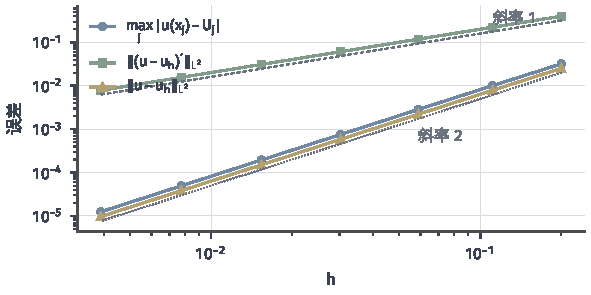
\includegraphics[width=100mm]{figures/03-optimization-evolution-and-signals/02-processes-and-trajectory-evolution/matplotlib/pde-convergence/figure.pdf}
  \caption{$-u''=\pi^2\sin(\pi x)$、两端为零时的误差随网格尺寸$h=1/(N+1)$的变化，$N=4,8,\ldots,256$，双对数坐标。蓝色：有限差分网格值的最大误差；绿色：有限元解导数的$L^2$误差；黄色：有限元解的$L^2$误差（载荷精确积分，单元上用$8$点Gauss求积计算误差）。灰色虚线与点线为斜率$1$与$2$的参考线。}
  \label{fig:pde-convergence}
\end{figure}

这两个阶都依赖$u\in H^2$。在高维的三角形网格上，类似的插值估计与Céa引理同样给出能量误差$O(h)$，但前提仍是解属于$H^2$；第~\ref{sec:pde-lax-milgram}小节L形区域凹角处的解不在$H^2$中，均匀网格上的收敛阶会相应降低，需要在凹角附近加密网格。误差阶来自“方程的稳定性（Céa引理）乘以解的可逼近性（插值估计）”，二者缺一不可。

\subsection{时间推进与误差分配}
\label{sec:pde-time-stepping}

\paragraph{半离散系统与刚性}
空间离散后的热方程是常微分方程组~\eqref{eq:pde-semidiscrete-heat}；有限元给出$\bm M\bm c'+\kappa\bm K\bm c=\bm F$，其中$\bm M_{i,j}=\langle\varphi_j,\varphi_i\rangle$是质量矩阵。矩阵$-\kappa\bm A_h$的特征值$-\kappa\mu_k$分布在约$-\kappa\pi^2$到$-4\kappa/h^2$之间，最快与最慢衰减率之比约为$4/(\pi^2h^2)$：$h=0.01$时约为$4000$。按第~\ref{chap:ordinary-differential-equations}章的说法，这是一个刚性问题：真正关心的是缓慢衰减的低频模式，最快的模式却限制了显式方法的步长。

\paragraph{显式Euler与扩散步长条件}
用步长$\Delta t$做显式Euler，$\bm U^{(n+1)}=\bm U^{(n)}-\Delta t\,\kappa\bm A_h\bm U^{(n)}$，逐点写出来是
\begin{equation}
  U_j^{(n+1)}=U_j^{(n)}+r\bigl(U_{j-1}^{(n)}-2U_j^{(n)}+U_{j+1}^{(n)}\bigr),\qquad r=\frac{\kappa\Delta t}{h^2} .
  \label{eq:pde-explicit-heat}
\end{equation}
第$k$个特征分量每步乘以放大因子$g_k=1-\Delta t\,\kappa\mu_k=1-4r\sin^2(k\pi h/2)$。所有分量不增长要求$|g_k|\leq1$，即$4r\sin^2(k\pi h/2)\leq2$对所有$k\leq N$成立；$r\leq1/2$时它对任何网格成立，而$h\to0$时$\sin^2(N\pi h/2)\to1$，所以$r$略大于$1/2$就会让最高频分量增长。这就是扩散问题显式格式的步长条件$\Delta t\leq h^2/(2\kappa)$。

$r\leq1/2$还有一个直接的读法：式~\eqref{eq:pde-explicit-heat}可写为$U_j^{(n+1)}=rU_{j-1}^{(n)}+(1-2r)U_j^{(n)}+rU_{j+1}^{(n)}$，三个系数非负且和为$1$，新值是旧值的凸组合，所以网格上的最大值不增、最小值不减，这是热方程最大值原理的离散版本。$r>1/2$时中间系数为负，凸组合的解释失效。图~\ref{fig:pde-explicit-stability}比较了$r=0.48$与$r=0.52$：初值是$\sin(\pi x)$加上振幅$0.01$的锯齿扰动，前者的锯齿迅速消失，后者的锯齿每步反号并放大，$60$步后最大值已约为$1.09$，而真解此时约为$0.46$。

\begin{figure*}[!htb]
  \centering
  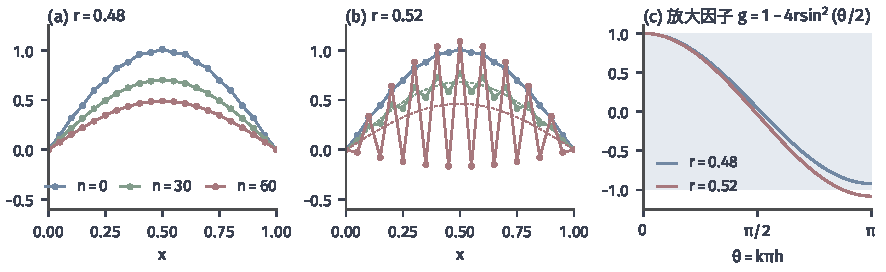
\includegraphics[width=150mm]{figures/03-optimization-evolution-and-signals/02-processes-and-trajectory-evolution/matplotlib/pde-explicit-stability/figure.pdf}
  \caption{热方程显式格式~\eqref{eq:pde-explicit-heat}的稳定与失稳，$h=1/20$，初值$\sin(\pi x_j)+0.01(-1)^j$。(a)~$r=0.48$：第$0,30,60$步的网格解（带点折线）紧贴同时刻的真解$e^{-\pi^2t}\sin(\pi x)$（同色虚线）。(b)~$r=0.52$：高频锯齿逐步放大，第$60$步最大值约$1.09$。(c)~放大因子$g=1-4r\sin^2(\theta/2)$随离散频率$\theta=k\pi h$的变化，浅蓝带为$|g|\leq1$；$r=0.52$的曲线在高频端越出$-1$。}
  \label{fig:pde-explicit-stability}
\end{figure*}

这个条件的代价随网格加细迅速增长：$h$减半，步长须缩为四分之一，总步数增为四倍，每步的工作量又增为两倍。限制步长的是稳定性，不是精度：$r\leq1/2$时，最高频模式无论如何都会被正确地衰减掉，却仍然决定了整个计算的步长。

\paragraph{隐式格式：后向Euler与梯形法}
后向Euler在新时刻计算导数：$(\bm I+\Delta t\,\kappa\bm A_h)\bm U^{(n+1)}=\bm U^{(n)}$。放大因子$g_k=1/(1+\Delta t\,\kappa\mu_k)\in(0,1)$对任何$\Delta t$都成立，格式无条件稳定，且对高频模式强烈衰减；代价是每步解一个三对角方程组，仍只需$O(N)$次运算。梯形法（在偏微分方程中常称Crank--Nicolson格式）取两端的平均，$g_k=(1-z_k/2)/(1+z_k/2)$，$z_k=\Delta t\,\kappa\mu_k$。它对所有$z_k\geq0$满足$|g_k|<1$，也无条件稳定，时间精度为二阶，而后向Euler只有一阶；但$z_k\to\infty$时$g_k\to-1$，步长较大时高频模式几乎不衰减、每步反号。所以“无条件稳定”不等于“强烈阻尼”，初值粗糙时梯形法的解可能出现长时间残留的小振荡。

\paragraph{波动方程与CFL条件}
对$u_{tt}=c^2u_{xx}$，时间与空间都用中心差商，得到跳蛙格式
\[
  U_j^{(n+1)}-2U_j^{(n)}+U_j^{(n-1)}=\nu^2\bigl(U_{j-1}^{(n)}-2U_j^{(n)}+U_{j+1}^{(n)}\bigr),\qquad\nu=\frac{c\Delta t}{h} .
\]
代入$U_j^{(n)}=g^n\sin(k\pi x_j)$，记$s=\sin^2(k\pi h/2)$，得$g^2-2(1-2\nu^2s)g+1=0$。两根之积为$1$。若$|1-2\nu^2s|\leq1$，两根是模为$1$的共轭复数（或重根），模式既不增长也不衰减，正如连续的波动方程保持能量；若$1-2\nu^2s<-1$，即$\nu^2s>1$，两根为实数且其中一个的绝对值大于$1$，模式指数增长。由于$s<1$，$\nu\leq1$保证所有模式稳定；而$h\to0$时最高频的$s\to1$，$\nu$略大于$1$就会失稳。$\nu\leq1$称为\term{CFL条件}（Courant--Friedrichs--Lewy condition）。

它有一个与第~\ref{sec:pde-wave-solution}小节相呼应的几何解释。跳蛙格式第$n$步在$x_j$处的值只依赖初始网格值在$[x_j-nh,x_j+nh]$中的部分，这是数值的依赖区域；真解依赖的是$[x_j-cn\Delta t,x_j+cn\Delta t]$。若$c\Delta t>h$，真解的依赖区域超出了数值的依赖区域，改变超出部分的初始数据会改变真解而不改变数值解，格式不可能收敛。所以数值依赖区域必须包含真解的依赖区域，这是收敛的必要条件。对输运方程$u_t+bu_x=0$（$b>0$），\term{迎风格式}（upwind scheme）$U_j^{(n+1)}=U_j^{(n)}-\nu(U_j^{(n)}-U_{j-1}^{(n)})$、$\nu=b\Delta t/h$，在$0\leq\nu\leq1$时是$U_{j-1}^{(n)}$与$U_j^{(n)}$的凸组合，因而稳定；改用下游的$U_{j+1}^{(n)}$则对任何$\nu>0$都不稳定，因为信息来自上游，这与第~\ref{sec:pde-characteristics}小节只在流入边界给数据是同一个道理。

\paragraph{误差分配}
在终止时刻，总误差可以拆成几部分：连续解与半离散解之差是空间误差，对二阶差分为$O(h^2)$；半离散解与时间推进结果之差是时间误差，后向Euler为$O(\Delta t)$、梯形法为$O(\Delta t^2)$；每步隐式方程只解到某个残差时，还有代数误差；此外是舍入误差。总误差不超过各部分之和，计算量则由网格点数与步数共同决定。

图~\ref{fig:pde-error-plateau}用一个可以精确计算的例子显示这种分配。取$u_t=u_{xx}$、两端为零、$u_0=\sin(\pi x)$，在$t=0.1$比较网格解与真解$e^{-\pi^2t}\sin(\pi x)$。由于$\sin(\pi x_j)$恰是$\bm A_h$的特征向量，所有误差都可以写成显式的标量公式。固定$h$，减小$\Delta t$时后向Euler的误差先按$\Delta t$线性下降，然后停在一个平台上：平台高度是空间误差，$h=1/10,1/20,1/40$时分别约为$3.0\times10^{-3}$、$7.6\times10^{-4}$、$1.9\times10^{-4}$，每次减半$h$降为约四分之一。到达平台后再减小$\Delta t$只是浪费计算。梯形法用大得多的步长就到达平台；它的曲线在某处出现向下的尖谷，是因为时间误差与空间误差符号相反、在那里恰好抵消，并不说明那个步长有特殊的精度。

\begin{figure}[!htb]
  \centering
  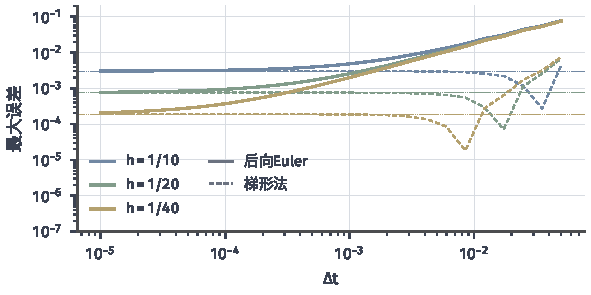
\includegraphics[width=100mm]{figures/03-optimization-evolution-and-signals/02-processes-and-trajectory-evolution/matplotlib/pde-error-plateau/figure.pdf}
  \caption{热方程$u_t=u_{xx}$、$u_0=\sin(\pi x)$在$t=0.1$时网格解的最大误差随时间步长的变化。三种颜色对应$h=1/10,1/20,1/40$；实线为后向Euler，虚线为梯形法；水平点线为同一$h$下半离散系统的空间误差。误差在$\Delta t$足够小后停在空间误差的平台上。}
  \label{fig:pde-error-plateau}
\end{figure}

两种误差平衡时计算量最省。后向Euler要让$O(\Delta t)$与$O(h^2)$相当，需取$\Delta t\sim h^2$，步数与显式格式的稳定限制同阶，只是现在是精度要求；梯形法只需$\Delta t\sim h$。网格加密一倍，前者的总工作量约增为八倍，后者约增为四倍。

最后是残差与误差的关系。迭代求解$\bm B\bm x=\bm b$时，常在残差$\bm r=\bm b-\bm B\tilde{\bm x}$足够小时停止；误差$\bm x-\tilde{\bm x}=\bm B^{-1}\bm r$，所以残差小能否推出误差小，取决于$\|\bm B^{-1}\|$。对后向Euler的矩阵$\bm I+\Delta t\,\kappa\bm A_h$，特征值不小于$1$，$\|\bm B^{-1}\|_2\leq1$，误差不超过残差；对Poisson矩阵，式~\eqref{eq:pde-fd-stability}给出最大范数下误差不超过残差的$1/8$。但若只控制相对残差，相对误差可能放大到条件数倍，而$\bm A_h$的条件数约为$4/(\pi^2h^2)$：$h=10^{-3}$时，$10^{-6}$的相对残差只保证约$0.4$的相对误差。残差小要经过相应的稳定估计，才能解释为解的误差小。
